\documentclass[shownotes,11pt, aspectratio=169]{beamer}

\usepackage{pgfpages}
% These slides also contain speaker notes. You can print just the slides,
% just the notes, or both, depending on the setting below. Comment out the want
% you want.
\setbeameroption{hide notes} % Only slide
%\setbeameroption{show only notes} % Only notes
%\setbeameroption{show notes on second screen=right} % Both

\usepackage{helvet}
\usepackage[default]{Fira Sans}
\usepackage{array}
\usepackage{caption}
%\usepackage[clean]{svg}
\usepackage{tikz}
\usepackage{verbatim}
\setbeamertemplate{note page}{\pagecolor{yellow!5}\insertnote}
\usetikzlibrary{positioning}
\usetikzlibrary{snakes}
\usetikzlibrary{calc}
\usetikzlibrary{arrows}
\usetikzlibrary{decorations.markings}
\usetikzlibrary{shapes.misc}
\usetikzlibrary{matrix,shapes,arrows,fit,tikzmark}
\usepackage{amsmath}
\usepackage{mathpazo}
\usepackage{hyperref}
\usepackage{lipsum}
\usepackage{multimedia}
\usepackage{graphicx}
\usepackage{multirow}
\usepackage{graphicx}
\usepackage{dcolumn}
\usepackage{bbm}
\usepackage{tfrupee}
\newcolumntype{d}[0]{D{.}{.}{5}}

\usepackage{changepage}
\usepackage{appendixnumberbeamer}
\newcommand{\beginbackup}{
   \newcounter{framenumbervorappendix}
   \setcounter{framenumbervorappendix}{\value{framenumber}}
   \setbeamertemplate{footline}
   {
     \leavevmode%
     \hline
     box{%
       \begin{beamercolorbox}[wd=\paperwidth,ht=2.25ex,dp=1ex,right]{footlinecolor}%
%         \insertframenumber  \hspace*{2ex} 
       \end{beamercolorbox}}%
     \vskip0pt%
   }
 }
\newcommand{\backupend}{
   \addtocounter{framenumbervorappendix}{-\value{framenumber}}
   \addtocounter{framenumber}{\value{framenumbervorappendix}} 
}


\usepackage{graphicx}
\usepackage[space]{grffile}
\usepackage{booktabs}

% These are my colors -- there are many like them, but these ones are mine.
\definecolor{blue}{RGB}{0,114,178}
\definecolor{red}{RGB}{213,94,0}
\definecolor{yellow}{RGB}{240,228,66}
\definecolor{green}{RGB}{0,158,115}
\definecolor{applegreen}{rgb}{0.55, 0.71, 0.0}
\definecolor{ao(english)}{rgb}{0.0, 0.5, 0.0}

\hypersetup{
  colorlinks=false,
  bookmarks=true,
  linkbordercolor = {white},
  linkcolor = {blue}
}


%% I use a beige off white for my background
\definecolor{MyBackground}{RGB}{255,253,218}

%% Uncomment this if you want to change the background color to something else
\setbeamercolor{background canvas}{bg=MyBackground}

%% Change the bg color to adjust your transition slide background color!
\newenvironment{transitionframe}{
  \setbeamercolor{background canvas}{bg=yellow}
  \begin{frame}}{
    \end{frame}
}

\setbeamercolor{frametitle}{fg=blue}
\setbeamercolor{title}{fg=black}
\setbeamertemplate{footline}[frame number]
\setbeamertemplate{navigation symbols}{} 
\setbeamertemplate{itemize items}{-}
\setbeamercolor{itemize item}{fg=blue}
\setbeamercolor{itemize subitem}{fg=blue}
\setbeamercolor{enumerate item}{fg=blue}
\setbeamercolor{enumerate subitem}{fg=blue}
\setbeamercolor{button}{bg=MyBackground,fg=blue,}



% If you like road maps, rather than having clutter at the top, have a roadmap show up at the end of each section 
% (and after your introduction)
% Uncomment this is if you want the roadmap!
% \AtBeginSection[]
% {
%    \begin{frame}
%        \frametitle{Roadmap of Talk}
%        \tableofcontents[currentsection]
%    \end{frame}
% }
\setbeamercolor{section in toc}{fg=blue}
\setbeamercolor{subsection in toc}{fg=red}
\setbeamersize{text margin left=1em,text margin right=1em} 

\newenvironment{wideitemize}{\itemize\addtolength{\itemsep}{10pt}}{\enditemize}

\title[]{\textcolor{blue}{Macroeconomics: Lecture 5}}
\author[SM]{Sumit Mishra}
\institute[IFMR]{\small{\begin{tabular}{c}
IFMR, Sri City \\
\end{tabular}}}

\date{08 October, 2019}


\begin{document}

%%% TIKZ STUFF
\tikzset{   
        every picture/.style={remember picture,baseline},
        every node/.style={anchor=base,align=center,outer sep=1.5pt},
        every path/.style={thick},
        }
\newcommand\marktopleft[1]{%
    \tikz[overlay,remember picture] 
        \node (marker-#1-a) at (-.3em,.3em) {};%
}
\newcommand\markbottomright[2]{%
    \tikz[overlay,remember picture] 
        \node (marker-#1-b) at (0em,0em) {};%
}
\tikzstyle{every picture}+=[remember picture] 
\tikzstyle{mybox} =[draw=black, very thick, rectangle, inner sep=10pt, inner ysep=20pt]
\tikzstyle{fancytitle} =[draw=black,fill=red, text=white]
%%%% END TIKZ STUFF

% Title Slide
\begin{frame}
\maketitle
%  \centering The views expressed do not necessarily reflect the position of the Federal Reserve Bank of New York or the Federal Reserve System.
\end{frame}

%%SLIDE 1
\begin{frame}
\frametitle{Agenda}
\begin{itemize}
\item Derive the aggregate supply curve, and the aggregate demand curve.
\item Determine the equilibrium in the short, and the medium run.
\item Dynamic Effects of Monetary/Fiscal Policy.
\item Material: Blanchard, Chapter 7.
\end{itemize}
\end{frame}

%%%%%%%%%%%%%%%%%%%%%%%%%%%%%%%%%%%%%%%%%%%%%%%%%%%%
\section{Aggregate Supply}
\begin{frame}
\begin{wideitemize}
\item $AS$ curve captures the effects of output on price level.
\item Recall the wage equation we derived in the last lecture.
      \[ W = P^eF(u,z) \]
\item Recap on the relationship between price level and wages.
     \[ P = (1 + m)W \]
\item We can now write the following \pause
     \[ P = (1 + m)P^eF(u,z) \]
\pause
\item Let me add more variables: \pause $u = \frac{U}{L} = 1 - \frac{N}{L} = 1 - \frac{Y}{L}$
\pause
\item $AS$ curve can be written as 
      \[ P = P^e(1 + m)F\Bigg(1 - \frac{Y}{L}, z\Bigg) \]           
\end{wideitemize}
\end{frame}


\begin{frame}{Aggregate Supply}
\textit{For a given expected price level, \textcolor{red}{$\uparrow Y \Rightarrow \uparrow P$}}. Let us break this down.

\begin{wideitemize}
\item $\uparrow \text{Output} \Rightarrow \uparrow \text{Employment}$ \pause
\item $\uparrow \text{Employment} \Rightarrow \downarrow \text{Unemployment Rate}$ \pause
\item $\downarrow \text{Unemployment Rate} \Rightarrow \uparrow \text{Nominal Wage}$ \pause
\item $\uparrow \text{Nominal Wage} \Rightarrow \uparrow \text{Price set by firms}$
\end{wideitemize}
\end{frame}

\begin{frame}{Aggregate Supply}
\textit{For any given unemployment level, \textcolor{red}{$\uparrow P^e \Rightarrow \uparrow P$}}.
What do you think is going on? \pause

\begin{wideitemize}
\item If prices are expected to be higher, wage setters would demand higher nominal wage.
\item $\uparrow W \Rightarrow \uparrow \text{Costs} \Rightarrow \uparrow\text{Prices set by firms} \Rightarrow \uparrow P$
\end{wideitemize}
\end{frame}

\begin{frame}{Aggregate Supply: Properties}
Three useful properties.

\begin{itemize}
\item[1] The aggregate supply curve is \textbf{upward sloping}.
\item[2] The $AS$ curve passes through a point such that $P=P^e$, $Y=Y_n$.
\item[3] $\uparrow P^e \Rightarrow \text{Upward shift in } AS$.
\end{itemize}
\end{frame}

\begin{frame}
\makebox[\linewidth][c]{
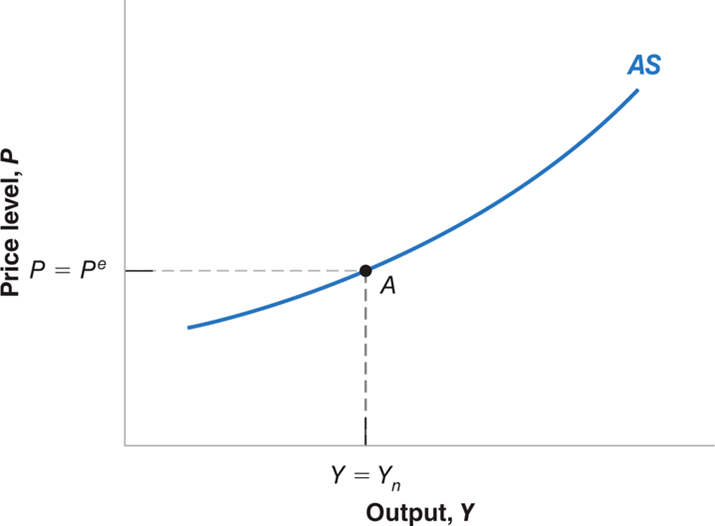
\includegraphics[scale=0.6]{graphs/L6F1.png}}
\end{frame}

\begin{frame}
\makebox[\linewidth][c]{
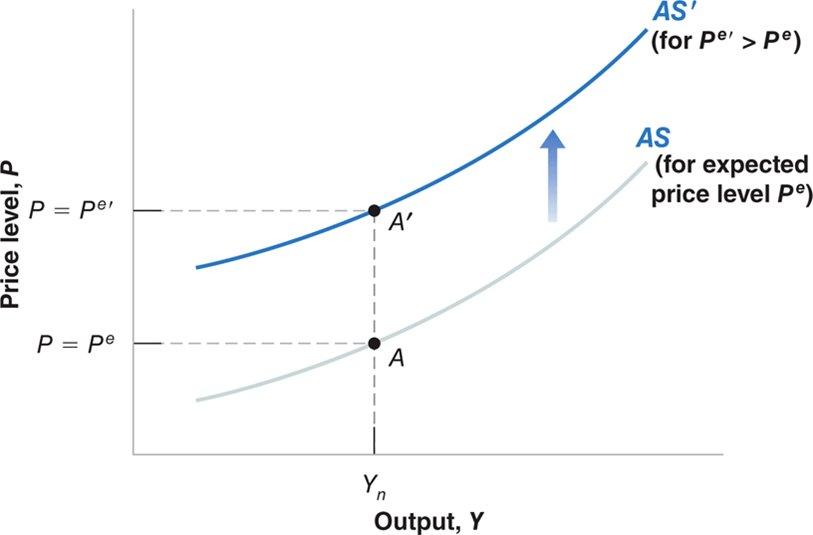
\includegraphics[scale=0.6]{graphs/L6F2.png}}
\end{frame}

%%%%%%%%%%%%%%%%%%%%%%%%%%%%%%%%%%%%%%%%%%%%%%%%%%%%5
\section{Aggregate Demand}

\begin{frame}{Aggregate Demand}
We will derive the aggregate demand relation using the $IS-LM$ framework.
\begin{itemize}
\item $IS$: \[Y = C(Y - T) + I(Y,i) + G \]
\item $LM$: \[ \frac{M}{P} = Y L(i) \] \pause
\item How does change in price level affect output? \pause
\item \textcolor{red}{$\uparrow P \Rightarrow \downarrow \frac{M}{P}$}
\end{itemize}
\end{frame}

\begin{frame}{Aggregate Demand}
Cookbook:

\begin{wideitemize}
\item Draw $IS$ and $LM$ curves.
\item Now, there is an increase in price level. Therefore, $\downarrow \frac{M}{P}$.
\item This would shift \pause $LM$ curve upwards. 
\item Equilibrium $ \uparrow i$, and $\downarrow Y$.
\item \textcolor{red}{$\uparrow P \Rightarrow \downarrow Y$}
\end{wideitemize}
\end{frame}

\begin{frame}
\makebox[\linewidth][c]{
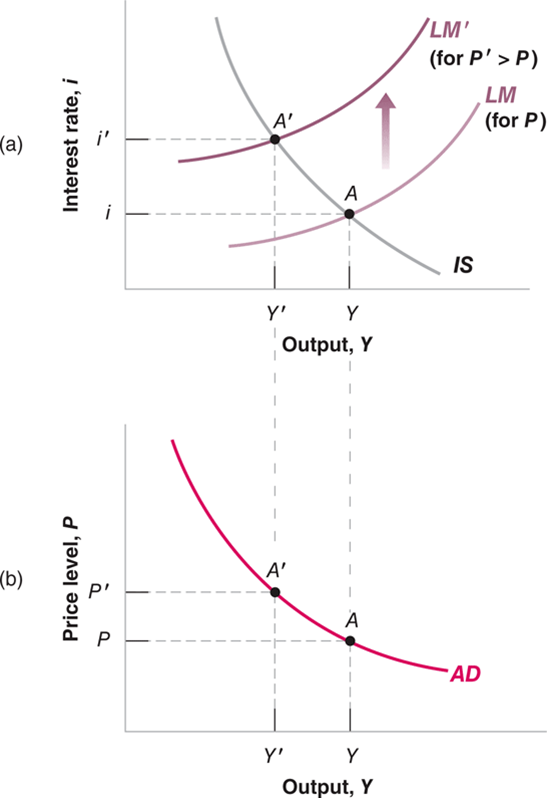
\includegraphics[scale=0.55]{graphs/L6F3.png}}
\end{frame}

\begin{frame}{Aggregate Demand}
\begin{columns}[T] % align columns
\begin{column}{.44\textwidth}
  \begin{wideitemize}
    \item Any variable that shifts $IS$ or $LM$ curve will shift the $AD$ function.
    \item $\uparrow G \Rightarrow AD \text{ shifts to the right}$.
    \item $\downarrow M \Rightarrow AD \text{ shifts to the left}$
    \item $AD$ function can be written as 
        \[ Y = Y\Bigg(\frac{M}{P}, G, T\Bigg) \]
  \end{wideitemize}
\end{column}%
\pause
\hfill%
\begin{column}{.53\textwidth}
  \makebox[\linewidth][c]{
    \resizebox{\linewidth}{!}{
      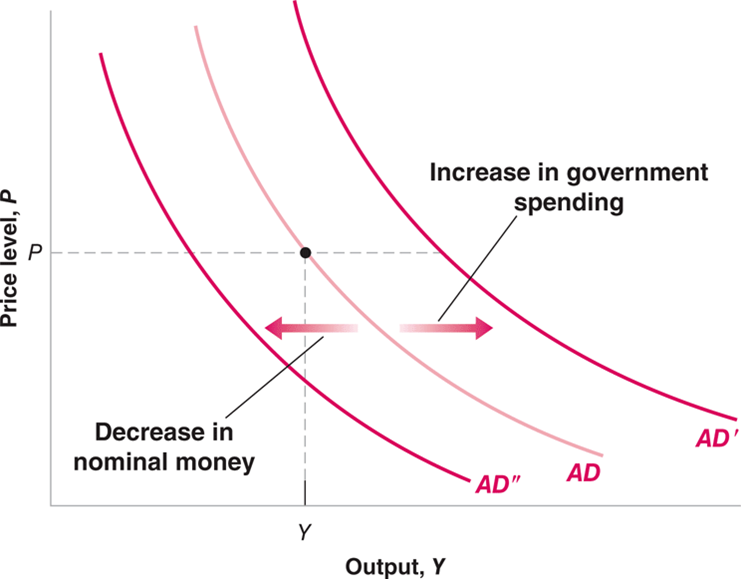
\includegraphics{graphs/L6F4.png}
    }
  }
\end{column}%
\end{columns}
\end{frame}

%%%%%%%%%%%%%%%%%%%%%%%%%%%%%%%%%%%%%%%%%%%%%%%%%%%%%%%%%%%%
\section{Equilibrium: Short and Medium Run}
\begin{frame}{Basic Set-up}
Recap:

\begin{itemize}
\item $AS$ Relation
      \[ P = P^e(1 + m)F\Bigg(1 - \frac{Y}{L}, z\Bigg) \]
\item $AD$ Relation
      \[ Y = Y\Bigg(\frac{M}{P}, G, T\Bigg) \]
\item The equilibrium depends upon $P^e$.
\item \textcolor{red}{In the short run, $P^e$ would be fixed}
\item \textcolor{red}{In the medium run, $P^e$ will change.}
\end{itemize}
\end{frame}


\begin{frame}{Short-Run Equilibrium}
\begin{columns}[T] % align columns
\begin{column}{.44\textwidth}
  \begin{wideitemize}
    \item An upward-sloping $AS$ curve.
    \item A downward-sloping $AD$ curve.
    \item $Y > Y_n$, and $P > P^e$.
  \end{wideitemize}
\end{column}%
\pause
\hfill%
\begin{column}{.53\textwidth}
  \makebox[\linewidth][c]{
    \resizebox{\linewidth}{!}{
      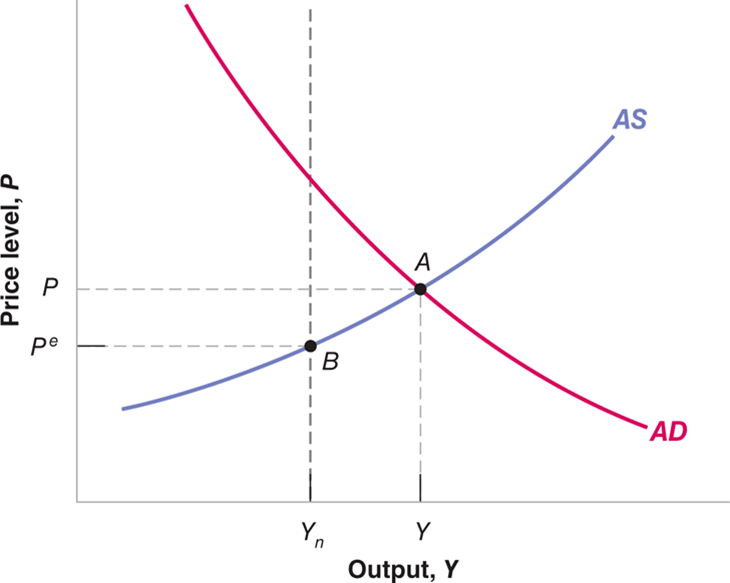
\includegraphics{graphs/L6F5.png}
    }
  }
\end{column}%
\end{columns}
What happens when time passes?
\end{frame}

\begin{frame}{From the Short Run to the Medium Run}
\begin{columns}[T] % align columns
\begin{column}{.44\textwidth}
  \begin{wideitemize}
    \item Since $P > P^e$, wage-setters would notice this and demand higher nominal wages.
    \item This would increase firms' wage bill (which would be transfered in form of higher prices).
    \item $AS$ curve will move upwards.
    \item Output will keep declining until it reaches the `natural' level.
    \item In the medium run, $Y = Y_n$ \& $P > P^e$.
  \end{wideitemize}
\end{column}%
\pause
\hfill%
\begin{column}{.53\textwidth}
  \makebox[\linewidth][c]{
    \resizebox{\linewidth}{!}{
      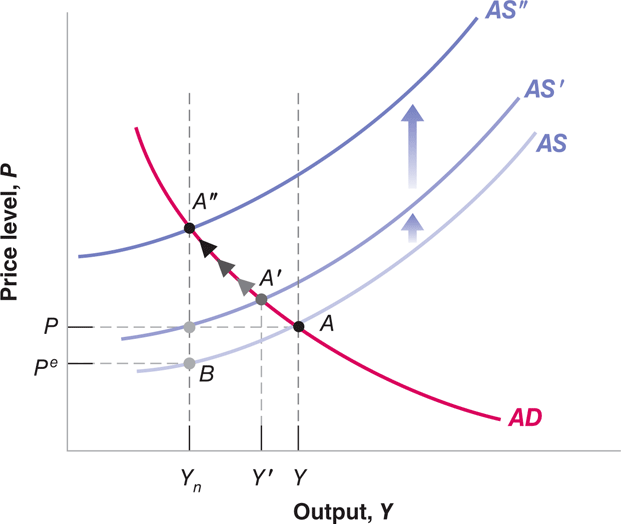
\includegraphics{graphs/L6F6.png}
    }
  }
\end{column}%
\end{columns}
\end{frame}

%%%%%%%%%%%%%%%%%%%%%%%%%%%%%%%%%%%%%%%%%
\section{The Effects of Monetary Expansion}
\begin{frame}
\textcolor{ao(english)}{Money suppy goes up.}
\begin{wideitemize}
\item What happens to $IS-LM$ curves? \pause The $LM$ curve shifts downwards. \pause
\item $AD$ curve shifts rightwards. \pause Output increases in the short run. \pause
\item Note that equilibrium price level is, now, also higher.
\item As time passes, price level will keep rising until...\pause
\item Output reaches the natural level.
\pause
\item $\uparrow P \Rightarrow \downarrow \frac{M}{P} \Rightarrow LM$ curve shifts upwards.
\end{wideitemize}
\vspace{2mm}

\textcolor{red}{Bottomline: \textit{The increase in nominal money is exactly offset by a proportional increase in the price level. The real money stock is therefore unchanged.}}
\end{frame}

\begin{frame}
  \makebox[\linewidth][c]{
    \resizebox{0.8\linewidth}{!}{
      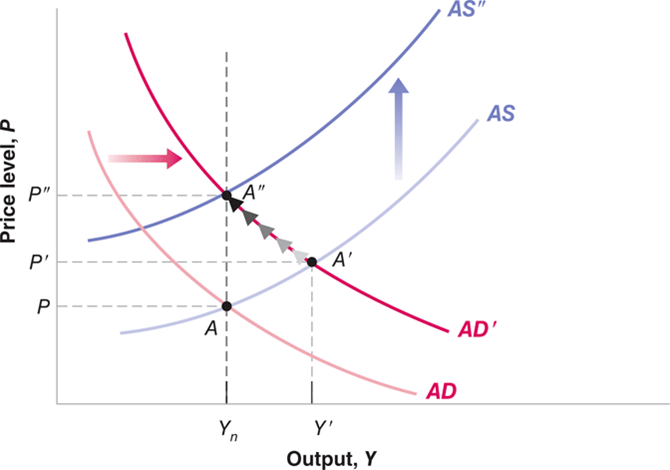
\includegraphics{graphs/L6F7.png}
    }
  }
\end{frame}

\begin{frame}
  \makebox[\linewidth][c]{
    \resizebox{0.4\linewidth}{!}{
      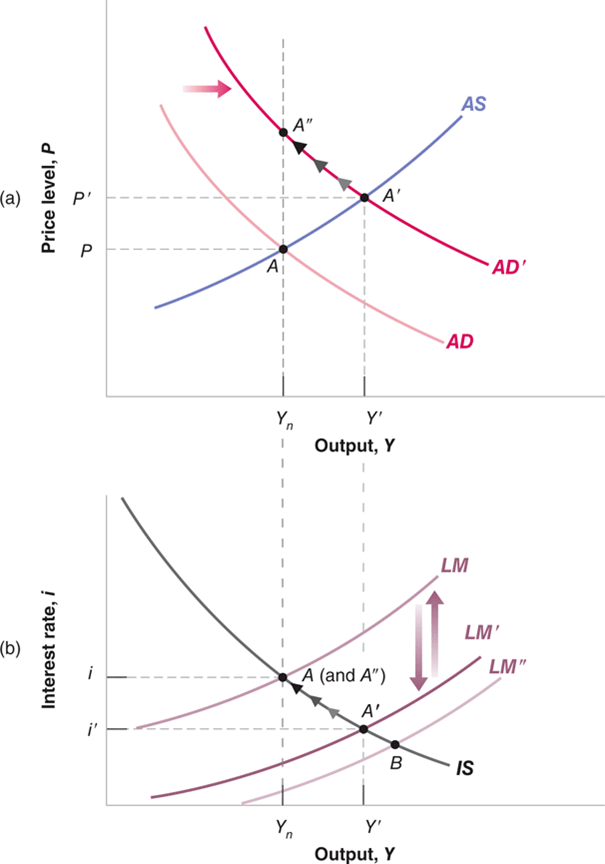
\includegraphics{graphs/L6F8.png}
    }
  }
\end{frame}

%%%%%%%%%%%%%%%%%%%%%%%%%%%%%%%%%%%%%%%%%
\section{The Effects of Reducing Deficit}
\begin{frame}{Budget Deficit Reduction}
\textcolor{green}{Government decides to cut some of its spendings.}
\begin{wideitemize}
\item There are two strategies: reduce $G$ or increase $T$. 
\item Suppose $\downarrow G \text{ and } \leftrightarrow T$.
\item Also suppose that $Y = Y_n$ at this point.
\pause
\item The $AD$ curve shifts leftwards. (\textbf{Reduction in output}).
\item Since output is below $Y_n$, the $AS$ will keep moving downwards until the economy is stabilized.
\end{wideitemize}
\end{frame}

\begin{frame}
  \makebox[\linewidth][c]{
    \resizebox{0.6\linewidth}{!}{
      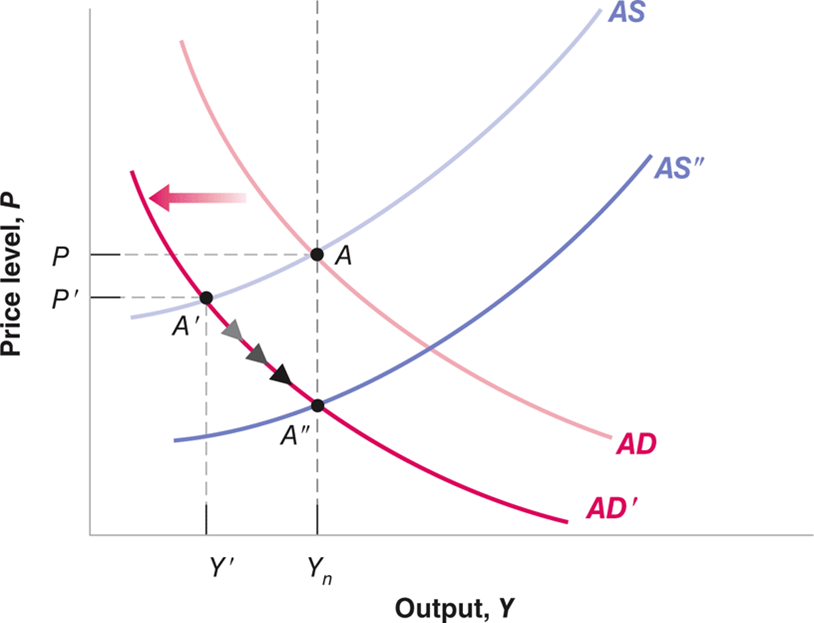
\includegraphics{graphs/L6F10.png}}
    }
\end{frame}

\begin{frame}{Deficit Reduction: Background Story}
\begin{wideitemize}
\item $\downarrow G \Rightarrow IS$ curve shifts leftwards. \pause
\item Now, recall that price level falls ($\downarrow P$). \pause 
\item What happens to the $LM$ curve? \pause
\item $\downarrow P \Rightarrow \uparrow \frac{M}{P}$
\item Fall in interest rate stops when $Y = Y_n$.
\pause
\item How is investment impacted in this process? 
\end{wideitemize}
\end{frame}

\begin{frame}{Deficit Reduction: Background Story-II}
\begin{wideitemize}
\item Let's go back to the start. 
      \begin{equation*} Y_n = C(Y_n - T) + I(Y_n,i) + G \end{equation*}
\item $\leftrightarrow Y \text{\&} T \Rightarrow \leftrightarrow C$
\item $\downarrow G$ has been compensated for by $\uparrow I$.
\end{wideitemize}
\end{frame}

\begin{frame}
  \makebox[\linewidth][c]{
    \resizebox{0.38\linewidth}{!}{
      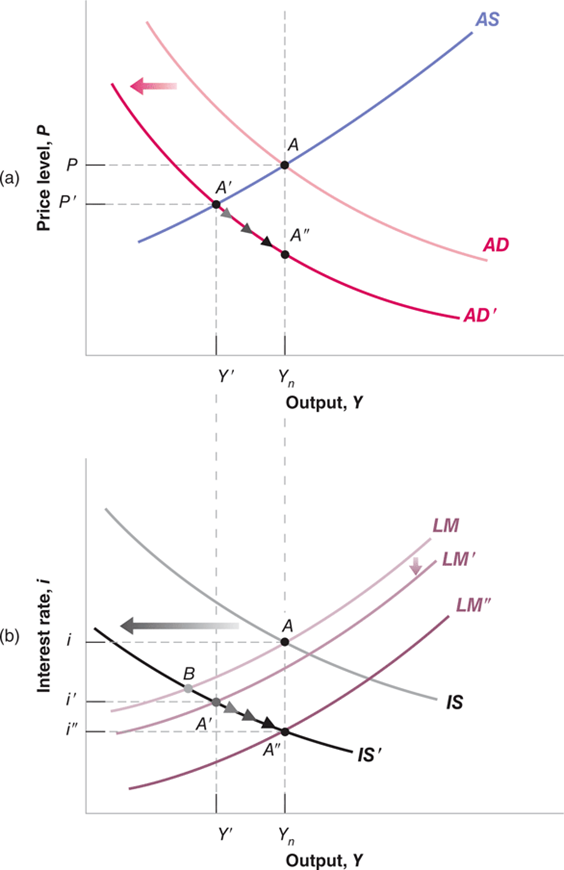
\includegraphics{graphs/L6F11.png}
    }
  }
\end{frame}

\begin{frame}{Deficit Reduction: Bottomline}
\begin{itemize}
\item[1] \textcolor{purple}{In the short run, a budget deficit reduction leads to a fall in investment and output.}
\pause
\vspace{6mm}
\item[2] \textcolor{ao(english)}{In the medium run, output returns to the natural level, and investments rise.}
\end{itemize}
\end{frame}

%%%%%%%%%%%%%%%%%%%%%%%%%%%%%%%%%%%%%%%%%%%%%%%%%%%%%%
\section{The Oil-Price Effects}
\begin{frame}{The Oil-Price Question}
\begin{itemize}
\item Formation of OPEC in the 1970s. 
\pause
\item Rise of China and other emerging economies put upward pressure on oil prices in the 2000s.
\pause
\item Our theoretical tools do not explicitly include oil prices, insofar.
\item Let's do that.
\pause
\item Link oil prices with the production of goods. 
\item $\uparrow \text{Oil Price } \Rightarrow \uparrow \text{ Cost of production}$.
\end{itemize}
\end{frame}

\begin{frame}{Effects on the Natural Rate of Unemployment}
Suppose that oil price has gone up.
\begin{columns}[T] % align columns
\begin{column}{.44\textwidth}
  \begin{wideitemize}
    \item Start think about labour market equilibrium.
    \item Increasing oil price will lead to a rise in cost of production.
    \item The price setting curve will move downwards because of rise in markup.
    \item The natural unemployment rate is now higher.
    \item Output will take a hit. 
  \end{wideitemize}
\end{column}%
\pause
\hfill%
\begin{column}{.53\textwidth}
  \makebox[\linewidth][c]{
    \resizebox{\linewidth}{!}{
      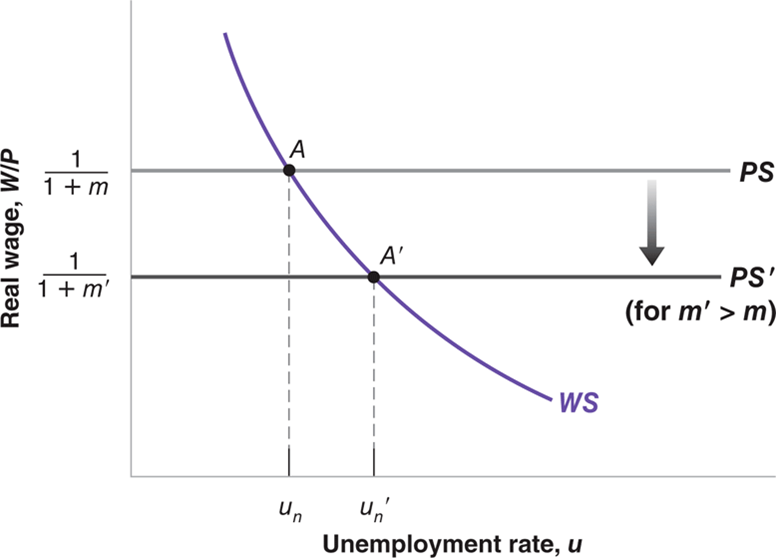
\includegraphics{graphs/L6F13.png}
    }
  }
\end{column}%
\end{columns}
\end{frame}

\begin{frame}{The Dynamics of Adjustment}
\begin{columns}[T] % align columns
\begin{column}{.44\textwidth}
  \begin{wideitemize}
    \item Output is now lower. Prices are higher. So, which way would the $AS$ curve move?
    \item $AS$ curve will move up.
    \item What happens over time? \pause
    \item It might just get worse.
  \end{wideitemize}
\end{column}%
\pause
\hfill%
\begin{column}{.53\textwidth}
  \makebox[\linewidth][c]{
    \resizebox{\linewidth}{!}{
      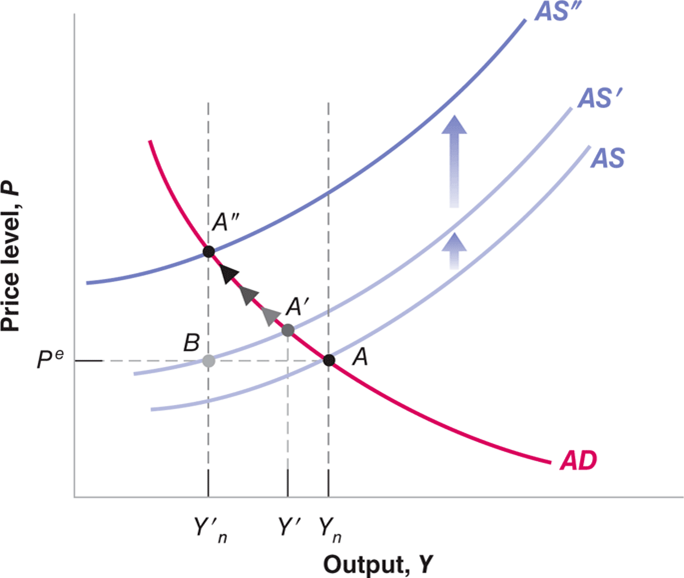
\includegraphics{graphs/L6F14.png}
    }
  }
\end{column}%
\end{columns}
\end{frame}

\begin{frame}{Cheatsheet}
 \makebox[\linewidth][c]{
    \resizebox{\linewidth}{!}{
      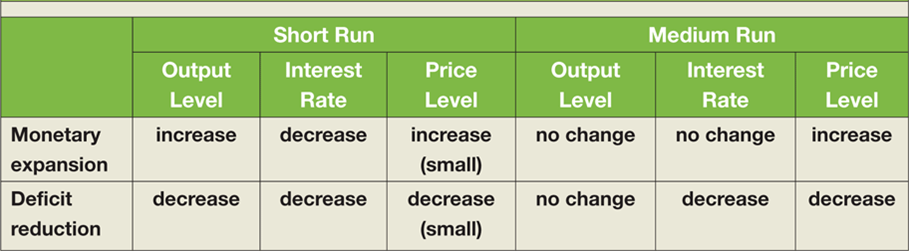
\includegraphics{graphs/L6F15.png}
    }
  }
\end{frame}

\end{document}
